
%%%%%%%%%%%%%%%%%%%%%%%%%%%%%%%%%%%%%%%%%%%%%%%%%%%%%
% ## Comparing media sentiment vs source bias
%%%%%%%%%%%%%%%%%%%%%%%%%%%%%%%%%%%%%%%%%%%%%%%%%%%%%

\begin{pyin}
import json
from matplotlib import pyplot as plt
import seaborn as sns
import pandas as pd
\end{pyin}

\begin{pyin}
\## load bias data ../data/documents_bias.json
ordinal_bias = ['Left', 'Left-Center', 'Least Biased', 'Right-Center', 'Right']
bias_text = {float(i+1): bias for i, bias in enumerate(ordinal_bias)}
bias_text[None] = None

with open('../data/documents_bias.json') as f:
    bias_data = {doc_id: bias_text[doc['bias_rating']] for doc_id, doc in json.load(f).items()}
\end{pyin}

\begin{pyin}
\## load sentiment data ../data/all_windows_classified.json
with open('../data/all_windows_classified.json') as f:
    instances = json.load(f)

ordinal_sentiment = ['positive', 'neutral', 'negative']
sentiment_data = {}

for instance_id, instance in instances.items():
    doc_id = instance_id.split('_')[0]
    sentiment = max(instance['sentiment'], key=instance['sentiment'].get)
    if doc_id not in sentiment_data:
        sentiment_data[doc_id] = []
    sentiment_data[doc_id].append(sentiment)
\end{pyin}

%%%%%%%%%%%%%%%%%%%%%%%%%%%%%%%%%%%%%%%%%%%%%%%%%%%%%
% ### Using Cross-Tabs
%%%%%%%%%%%%%%%%%%%%%%%%%%%%%%%%%%%%%%%%%%%%%%%%%%%%%

\begin{pyin}
\## Convert the first dictionary to a DataFrame
bias_df = pd.DataFrame(list(bias_data.items()), columns=['id', 'bias'])
bias_df['bias'] = pd.Categorical(bias_df['bias'], categories=ordinal_bias, ordered=True)

# Flatten the second dictionary and convert it to a DataFrame
sentiment_df = pd.DataFrame([(k, v) for k, vals in sentiment_data.items() for v in vals],
                            columns=['id', 'sentiment'])
sentiment_df['sentiment'] = pd.Categorical(sentiment_df['sentiment'], categories=ordinal_sentiment, ordered=True)

# Merge the two DataFrames on the 'id' column
merged_df = pd.merge(bias_df, sentiment_df, on='id', how='inner')

# Create a cross-tabulation of ordinal values and sentiment labels
crosstab = pd.crosstab(merged_df['sentiment'], merged_df['bias'])

# Print the cross-tabulation
print(crosstab)
\end{pyin}

\begin{pyprint}
bias       Left  Left-Center  Least Biased  Right-Center  Right
sentiment                                                      
positive     66          167           167            66     64
neutral     137          240           237           147    143
negative     30           94            40            37     88
\end{pyprint}

\begin{pyin}
\## Create a heatmap of the cross-tabulation
sns.heatmap(crosstab, annot=True, cmap="YlGnBu", cbar=True)

# Add labels and title
plt.xlabel('Sentiment')
plt.ylabel('Source Bias')
plt.title('Cross-tabulation of Ordinal Values and Sentiment Labels')

# Show the plot
plt.show()
\end{pyin}

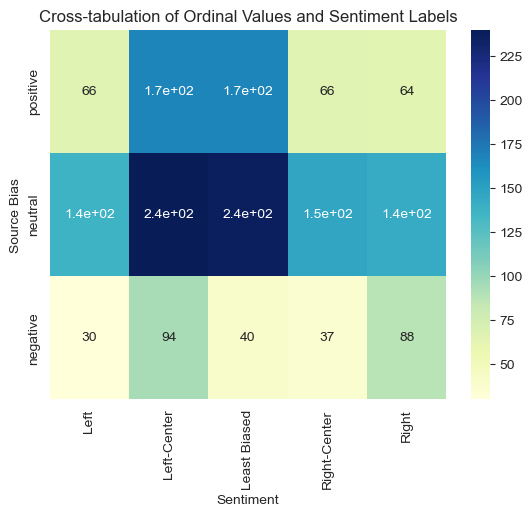
\includegraphics[width=\textwidth]{./figs/fig_2.png}
\begin{pyin}
\## Calculate proportions by normalizing the values in each row
crosstab_normalized = crosstab.div(crosstab.sum(axis=0), axis=1)

# Print the normalized cross-tabulation (proportions)
print(crosstab_normalized)

# Create a heatmap of the normalized cross-tabulation (proportions)
sns.heatmap(crosstab_normalized, annot=True, cmap="YlGnBu", cbar=True, fmt=".2f")

# Add labels and title
plt.xlabel('Source Bias')
plt.ylabel('Sentiment')
plt.title('Proportions of Sentiment Labels by Source Bias')

# Show the plot
plt.show()
\end{pyin}

\begin{pyprint}
bias           Left  Left-Center  Least Biased  Right-Center     Right
sentiment                                                             
positive   0.283262     0.333333      0.376126         0.264  0.216949
neutral    0.587983     0.479042      0.533784         0.588  0.484746
negative   0.128755     0.187625      0.090090         0.148  0.298305
\end{pyprint}

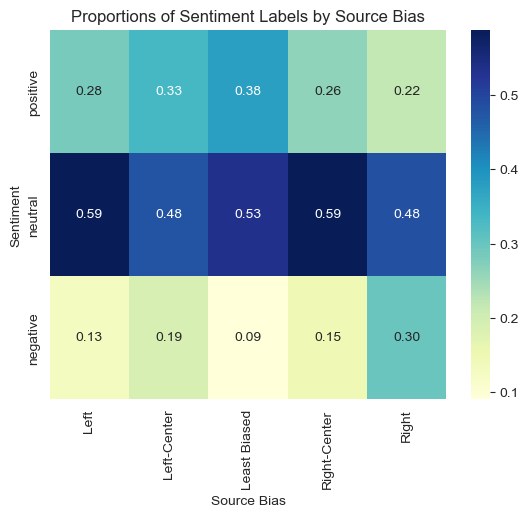
\includegraphics[width=\textwidth]{./figs/fig_3.png}
%%%%%%%%%%%%%%%%%%%%%%%%%%%%%%%%%%%%%%%%%%%%%%%%%%%%%
% ### Using Random Forests
%%%%%%%%%%%%%%%%%%%%%%%%%%%%%%%%%%%%%%%%%%%%%%%%%%%%%

\begin{pyin}
\## Get date information
with open('../data/documents_bias.json') as f:
    date_data = {doc_id: doc['date'] for doc_id, doc in json.load(f).items()}

# Add the date information to the bias_df DataFrame
bias_df['date'] = bias_df['id'].map(date_data)

# Convert the date column to a datetime object and extract year, month, and day
bias_df['date'] = pd.to_datetime(bias_df['date'])
bias_df['year'] = bias_df['date'].dt.year
bias_df['month'] = bias_df['date'].dt.month
bias_df['day'] = bias_df['date'].dt.day
\end{pyin}

\begin{pyin}
from sklearn.ensemble import RandomForestClassifier
from sklearn.preprocessing import LabelEncoder
from sklearn.model_selection import train_test_split, GridSearchCV
from sklearn.metrics import classification_report
from imblearn.over_sampling import RandomOverSampler

# Merge the bias_df and sentiment_df DataFrames (as in previous code)
df = pd.merge(bias_df, sentiment_df, on='id', how='inner')

# Encode the 'bias' and 'sentiment' columns using LabelEncoder
label_encoder_bias = LabelEncoder()
label_encoder_sentiment = LabelEncoder()
df['bias_encoded'] = label_encoder_bias.fit_transform(df['bias'])
df['sentiment_encoded'] = label_encoder_sentiment.fit_transform(df['sentiment'])

# Add the date components (year, month, day) to the independent variables
X = df[['bias_encoded', 'year', 'month', 'day']]
y = df['sentiment_encoded']

# Split the data into training and testing sets
X_train, X_test, y_train, y_test = train_test_split(
    X,  # Independent variables (source bias and date components)
    y,  # Dependent variable (sentiment)
    test_size=0.2,
    random_state=42
)

# Apply RandomOverSampler to oversample minority classes in the training set
ros = RandomOverSampler(random_state=42)
X_train_resampled, y_train_resampled = ros.fit_resample(X_train, y_train)

# Initialize the Random Forest Classifier
rf_clf = RandomForestClassifier(random_state=42)

# Define the hyperparameter grid to search over
param_grid = {
    'n_estimators': [50, 100, 200],
    'max_depth': [None, 10, 20],
    'min_samples_split': [2, 5, 10]
}

# Initialize GridSearchCV with the Random Forest Classifier and the hyperparameter grid
grid_search = GridSearchCV(rf_clf, param_grid, cv=5, scoring='accuracy')

# Train the model on the resampled training data and perform hyperparameter tuning
grid_search.fit(X_train_resampled, y_train_resampled)

# Print the best hyperparameters
print("Best Hyperparameters:", grid_search.best_params_)

# Use the best model found by GridSearchCV to make predictions on the testing data
best_rf_clf = grid_search.best_estimator_
y_pred = best_rf_clf.predict(X_test)

# Evaluate the model's performance
print(classification_report(y_test, y_pred, target_names=ordinal_sentiment))
\end{pyin}

\begin{pyprint}
Best Hyperparameters: {'max_depth': 20, 'min_samples_split': 2, 'n_estimators': 200}
              precision    recall  f1-score   support

    positive       0.30      0.60      0.40       112
     neutral       0.72      0.55      0.63       534
    negative       0.52      0.55      0.53       297

    accuracy                           0.56       943
   macro avg       0.52      0.57      0.52       943
weighted avg       0.61      0.56      0.57       943
\end{pyprint}

%%%%%%%%%%%%%%%%%%%%%%%%%%%%%%%%%%%%%%%%%%%%%%%%%%%%%
% ## Frequency of Coverage by Source Bias
%%%%%%%%%%%%%%%%%%%%%%%%%%%%%%%%%%%%%%%%%%%%%%%%%%%%%

\begin{pyin}
\## Define the desired order of the bias categories
bias_order = ["Left", "Left-Center", "Least Biased", "Right-Center", "Right"]

# Convert the 'bias' column to a categorical data type with the specified order
bias_df['bias'] = pd.Categorical(bias_df['bias'], categories=bias_order, ordered=True)

# Create the bar chart with the frequency of coverage by source bias
# The bars will be ordered based on the specified order of categories
bias_df['bias'].value_counts(sort=False).plot(kind='bar')
plt.title('Frequency of Coverage by Source Bias')
plt.xlabel('Source Bias')
plt.ylabel('Frequency')
plt.show()
\end{pyin}

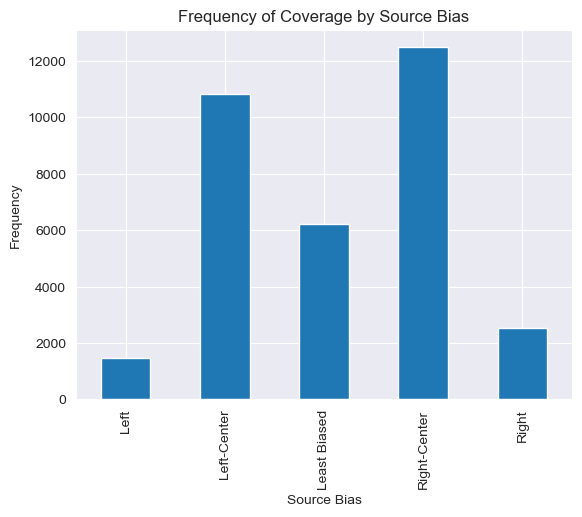
\includegraphics[width=\textwidth]{./figs/fig_4.png}
\begin{pyin}
\## Assuming bias_df contains 'date', 'bias', and 'id' columns
# 'date' - the date associated with each document
# 'bias' - the source bias category for each document
# 'id' - the unique identifier for each document

# Group the data by both date and bias category, and count the frequency of coverage for each group
coverage_by_date_bias = bias_df.groupby(['date', 'bias']).size().reset_index(name='frequency')

# Pivot the data to create a DataFrame with date as the index and bias categories as columns
coverage_pivot = coverage_by_date_bias.pivot(index='date', columns='bias', values='frequency').fillna(0)

# Sort the DataFrame by date
coverage_pivot.sort_index(inplace=True)

# Resample the data into monthly intervals and sum the frequencies within each interval
coverage_resampled = coverage_pivot.resample('W').sum()

# Plot the stacked line chart
ax = coverage_resampled.plot(kind='line', stacked=True, figsize=(12, 8))

# Add labels and title
ax.set_xlabel('Date')
ax.set_ylabel('Frequency of Coverage')
ax.set_title('Frequency of Coverage by Source Bias Over Time (Weekly)')

# Show the plot
plt.tight_layout()
plt.show()

\end{pyin}

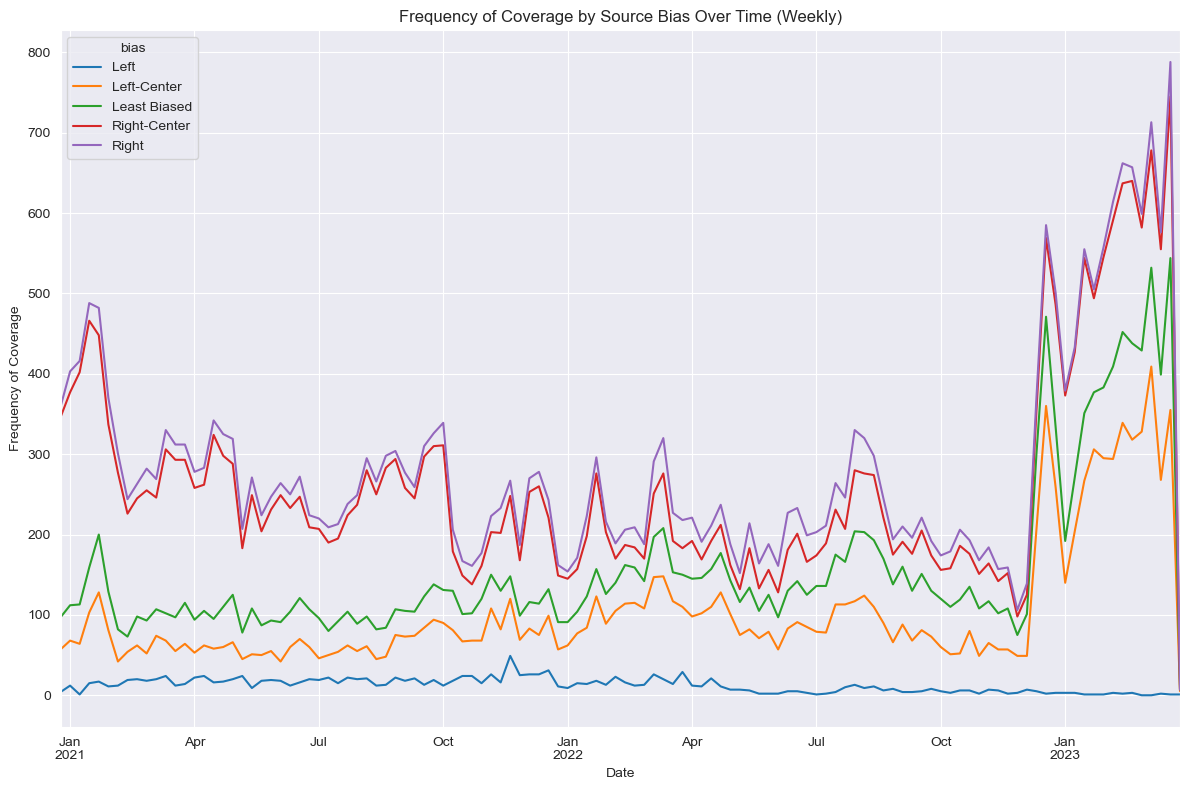
\includegraphics[width=\textwidth]{./figs/fig_5.png}
%%%%%%%%%%%%%%%%%%%%%%%%%%%%%%%%%%%%%%%%%%%%%%%%%%%%%
% #### Now let's look at the same data, but with important dates highlighted
%%%%%%%%%%%%%%%%%%%%%%%%%%%%%%%%%%%%%%%%%%%%%%%%%%%%%

\begin{pyin}
\## Create a list of important dates from ../data/bill_data.json
with open('../data/bill_data.json') as f:
    bill_data = json.load(f)

bill_introduced_dates = [bill['introduced'] for bill in bill_data.values()]
last_action_dates_unix = [bill['last_action_timestamp'] for bill in bill_data.values()]
\end{pyin}

\begin{pyin}
\## Plot the stacked line chart
ax = coverage_resampled.plot(kind='line', stacked=True, figsize=(12, 8))

# Add labels and title
ax.set_xlabel('Date')
ax.set_ylabel('Frequency of Coverage')
ax.set_title('Frequency of Coverage by Source Bias Over Time (Weekly)')

# Add vertical lines for bill introduced dates
for date in bill_introduced_dates:
    ax.axvline(pd.Timestamp(date), color='red', linestyle='--')

# Add vertical lines for last action dates (convert Unix timestamps to datetime objects)
for unix_timestamp in last_action_dates_unix:
    date = pd.Timestamp(unix_timestamp, unit='s')
    ax.axvline(date, color='blue', linestyle='--')

# Add a legend to the plot (bbox_to_anchor and loc adjust the legend position to avoid overlap)
ax.legend(bbox_to_anchor=(1.05, 1), loc='upper left')

# Show the plot
plt.tight_layout()
plt.show()
\end{pyin}

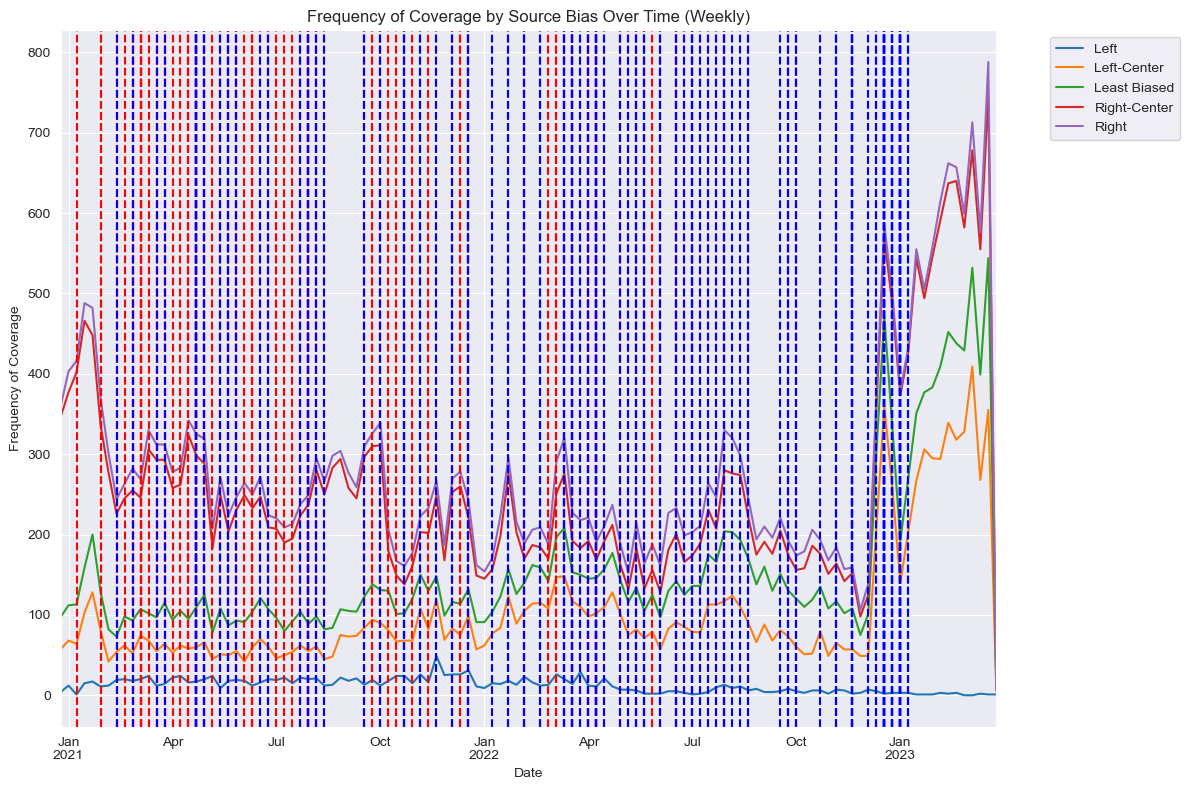
\includegraphics[width=\textwidth]{./figs/fig_6.png}
%%%%%%%%%%%%%%%%%%%%%%%%%%%%%%%%%%%%%%%%%%%%%%%%%%%%%
% #### Hmmmm.... that's too many dates. Let's just look at the top 3 most frequent bills? Later though.
%%%%%%%%%%%%%%%%%%%%%%%%%%%%%%%%%%%%%%%%%%%%%%%%%%%%%

%%%%%%%%%%%%%%%%%%%%%%%%%%%%%%%%%%%%%%%%%%%%%%%%%%%%%
% ### Let's see what periods have the most coverage from each category
%%%%%%%%%%%%%%%%%%%%%%%%%%%%%%%%%%%%%%%%%%%%%%%%%%%%%

\begin{pyin}
\## Find the week with the highest coverage for each bias category
max_coverage_weeks = coverage_resampled.idxmax()

# Print the results
for bias, week in max_coverage_weeks.items():
    coverage = coverage_resampled.loc[week, bias]
    print(f"'{bias}': {coverage} -> {week}")
\end{pyin}

\begin{pyprint}
'Left': 49 -> 2021-11-21 00:00:00+00:00
'Left-Center': 409 -> 2023-03-05 00:00:00+00:00
'Least Biased': 189 -> 2023-03-19 00:00:00+00:00
'Right-Center': 307 -> 2021-01-17 00:00:00+00:00
'Right': 50 -> 2022-07-31 00:00:00+00:00
\end{pyprint}

%%%%%%%%%%%%%%%%%%%%%%%%%%%%%%%%%%%%%%%%%%%%%%%%%%%%%
% ### Now let's see what bills were introduced or had their last action during these periods
%%%%%%%%%%%%%%%%%%%%%%%%%%%%%%%%%%%%%%%%%%%%%%%%%%%%%

\begin{pyin}
\## Convert bill_introduced_dates and last_action_dates_unix to Pandas Timestamps
bill_introduced_dates = pd.to_datetime(bill_introduced_dates).tz_localize(None)
last_action_dates_unix = pd.to_datetime(last_action_dates_unix, unit='s').tz_localize(None)

# Initialize lists to store the introduced and last action dates that fall within the periods
introduced_dates_in_period = []
last_action_dates_in_period = []

# Check if the dates fall within the periods
for bias, week in max_coverage_weeks.items():
    coverage = coverage_resampled.loc[week, bias]
    print(f"'{bias}': {coverage} -> {week}")

    # Calculate the start and end dates of the period (week), and remove time zone information
    start_date = week.tz_localize(None)
    end_date = (week + pd.DateOffset(weeks=1)).tz_localize(None)

    # Check if bill_introduced_dates are within the period
    for date in bill_introduced_dates:
        if start_date <= date < end_date:
            introduced_dates_in_period.append(date)

    # Check if last_action_dates_unix are within the period
    for date in last_action_dates_unix:
        if start_date <= date < end_date:
            last_action_dates_in_period.append(date)

# Print the results
print("Bill introduced dates within the periods:", introduced_dates_in_period)
print("Last action dates within the periods:", last_action_dates_in_period)
\end{pyin}

\begin{pyprint}
'Left': 49 -> 2021-11-21 00:00:00+00:00
'Left-Center': 409 -> 2023-03-05 00:00:00+00:00
'Least Biased': 189 -> 2023-03-19 00:00:00+00:00
'Right-Center': 307 -> 2021-01-17 00:00:00+00:00
'Right': 50 -> 2022-07-31 00:00:00+00:00
Bill introduced dates within the periods: []
Last action dates within the periods: [Timestamp('2022-08-02 06:00:00')]
\end{pyprint}

\begin{pyin}
\## TODO: There's more to do here :)
\end{pyin}

%%%%%%%%%%%%%%%%%%%%%%%%%%%%%%%%%%%%%%%%%%%%%%%%%%%%%
% ### Let's just look at sentiment over time.
%%%%%%%%%%%%%%%%%%%%%%%%%%%%%%%%%%%%%%%%%%%%%%%%%%%%%

\begin{pyin}
\## Merge sentiment_df with date information from bias_df
merged_sentiment_df = pd.merge(sentiment_df, bias_df[['id', 'date']], on='id', how='inner')

# Convert the 'sentiment' column to a categorical variable with order
ordinal_sentiment = ['positive', 'neutral', 'negative']
merged_sentiment_df['sentiment'] = pd.Categorical(merged_sentiment_df['sentiment'], categories=ordinal_sentiment, ordered=True)

# Set 'date' as the DataFrame's index
merged_sentiment_df.set_index('date', inplace=True)

# Resample the data by month (or any other frequency of your choice)
sentiment_resampled = merged_sentiment_df.resample('M')

# Count sentiment frequencies for each month
sentiment_counts = sentiment_resampled['sentiment'].value_counts().unstack().fillna(0)

# Plot the stacked line chart showing sentiment frequencies over time
sentiment_counts.plot(kind='line')
plt.xlabel('Date')
plt.ylabel('Sentiment Frequency')
plt.title('Sentiment Frequency Over Time')
plt.legend(title='Sentiment')
plt.show()

\end{pyin}

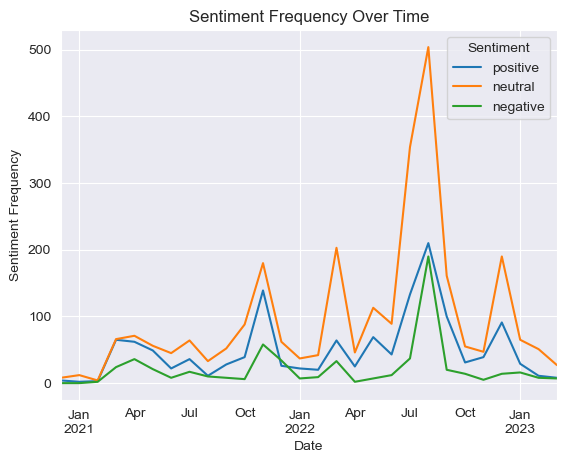
\includegraphics[width=\textwidth]{./figs/fig_7.png}
\begin{pyin}
\## Merge sentiment_df with date information from bias_df
merged_sentiment_df = pd.merge(sentiment_df, bias_df[['id', 'date']], on='id', how='inner')

# Convert the 'sentiment' column to numerical scores
sentiment_scores = {'positive': 1, 'neutral': 0, 'negative': -1}
merged_sentiment_df['sentiment_score'] = merged_sentiment_df['sentiment'].map(sentiment_scores).astype(float)

# Set 'date' as the DataFrame's index
merged_sentiment_df.set_index('date', inplace=True)

# Resample the data by month (or any other frequency of your choice) and calculate the mean sentiment score
sentiment_resampled = merged_sentiment_df.resample('M')['sentiment_score'].mean()

# Create the heatmap
fig, ax = plt.subplots(figsize=(12, 4))
sns.heatmap(sentiment_resampled.to_frame().T, cmap='RdBu_r', center=0, annot=True, fmt=".2f", cbar=True, ax=ax)

# Set the x-axis tick labels to match the dates in the sentiment_resampled DataFrame
ax.set_xticklabels([date.strftime('%b %Y') for date in sentiment_resampled.index])

# Add labels and title
plt.xlabel('Date')
plt.ylabel('Sentiment')
plt.title('Sentiment Heatmap Over Time')

# Show the plot
plt.tight_layout()
plt.show()
\end{pyin}

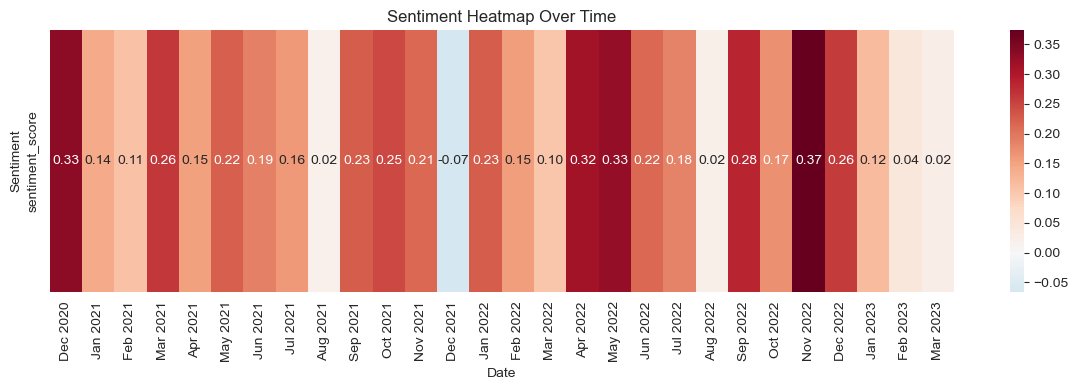
\includegraphics[width=\textwidth]{./figs/fig_8.png}
\begin{pyin}
\## Convert the bill_data dictionary to a DataFrame
bill_df = pd.DataFrame(bill_data.values())

# Convert the 'last_action_timestamp' column to a datetime object
bill_df['last_action_date'] = pd.to_datetime(bill_df['last_action_timestamp'], unit='s')

# Set 'last_action_date' as the DataFrame's index
bill_df.set_index('last_action_date', inplace=True)

# Resample the bill data by month (or any other frequency of your choice) and calculate the mean bill success
bill_success_resampled = bill_df.resample('M')['last_action_ordinal'].mean()

# Merge sentiment_df with date information from bias_df
merged_sentiment_df = pd.merge(sentiment_df, bias_df[['id', 'date']], on='id', how='inner')

# Set 'date' as the DataFrame's index
merged_sentiment_df.set_index('date', inplace=True)

# Resample the data by month and calculate the proportion of sentiment that is positive
sentiment_counts = merged_sentiment_df.resample('M')['sentiment'].value_counts().unstack().fillna(0)
positive_proportion = sentiment_counts['positive'] / sentiment_counts.sum(axis=1)

# Create the dual-axis plot
fig, ax1 = plt.subplots()
ax2 = ax1.twinx()

# Plot the proportion of positive sentiment on the left y-axis
positive_proportion.plot(kind='line', color='blue', ax=ax1, label='Proportion of Positive Sentiment')

# Plot the bill success on the right y-axis
bill_success_resampled.plot(kind='line', color='red', ax=ax2, label='Bill Success')

# Add labels, legend, and title
ax1.set_xlabel('Date')
ax1.set_ylabel('Proportion of Positive Sentiment', color='blue')
ax2.set_ylabel('Bill Success', color='red')
ax1.set_title('Proportion of Positive Sentiment and Bill Success Over Time')

# Add legends for both y-axes
ax1.legend(loc='upper left')
ax2.legend(loc='upper right')

# Show the plot
plt.show()

\end{pyin}

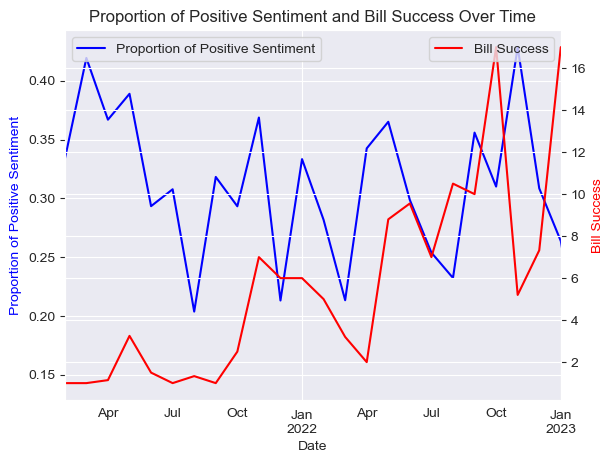
\includegraphics[width=\textwidth]{./figs/fig_9.png}
\begin{pyin}
\## Convert bill_data into a DataFrame
bill_df = pd.DataFrame(bill_data.values())

# Convert the last_action_timestamp to datetime and set it as the index
bill_df['last_action_date'] = pd.to_datetime(bill_df['last_action_timestamp'], unit='s')
bill_df.set_index('last_action_date', inplace=True)

# Resample the bill data by month and calculate the average success metric
bill_success = bill_df.resample('M')['last_action_ordinal'].mean()

# Define the bias categories and their corresponding names
bias_category_names = ['Left', 'Center', 'Right']

# Merge sentiment_df with date and bias information from bias_df
merged_sentiment_df = pd.merge(sentiment_df, bias_df[['id', 'date', 'bias_label']], on='id', how='inner')

# Set 'date' as the DataFrame's index
merged_sentiment_df.set_index('date', inplace=True)

# Create subplots with 3 rows and 1 column
fig, axes = plt.subplots(nrows=3, ncols=1, figsize=(10, 15))
fig.tight_layout(pad=5)

# Plot each bias category
for i, bias_category_name in enumerate(bias_category_names):
    # Filter the data based on the source bias category
    filtered_df = merged_sentiment_df[merged_sentiment_df['bias_label'] == bias_category_name]
    num_data_points = filtered_df.shape[0]
    print(f"Number of data points for {bias_category_name} bias category: {num_data_points}")

    # Check if there are data points available
    if num_data_points > 0:
        # Resample the data by month and calculate the proportion of sentiment that is positive
        sentiment_counts = (filtered_df.groupby([pd.Grouper(freq='M'), 'sentiment'])
                            .size().unstack().fillna(0))
        positive_proportion = sentiment_counts.get('positive', 0) / sentiment_counts.sum(axis=1)

        # Plot the proportion of positive sentiment
        ax = axes[i]
        positive_proportion.plot(kind='line', color='blue', ax=ax, label='Proportion of Positive Sentiment')

        # Add the bill success line to the plot with a dual axis
        ax2 = ax.twinx()
        bill_success.plot(kind='line', color='red', ax=ax2, label='Bill Success')

        # Add labels and title
        ax.set_xlabel('Date')
        ax.set_ylabel('Proportion of Positive Sentiment')
        ax.set_title(f'Proportion of Positive Sentiment for {bias_category_name} Source Bias')
        ax2.set_ylabel('Bill Success')

        # Combine the legends
        lines, labels = ax.get_legend_handles_labels()
        lines2, labels2 = ax2.get_legend_handles_labels()
        ax.legend(lines + lines2, labels + labels2, loc='upper left')

# Show the plots
plt.show()

\end{pyin}

\begin{pyprint}
Number of data points for Left bias category: 233
Number of data points for Center bias category: 444
Number of data points for Right bias category: 295
\end{pyprint}

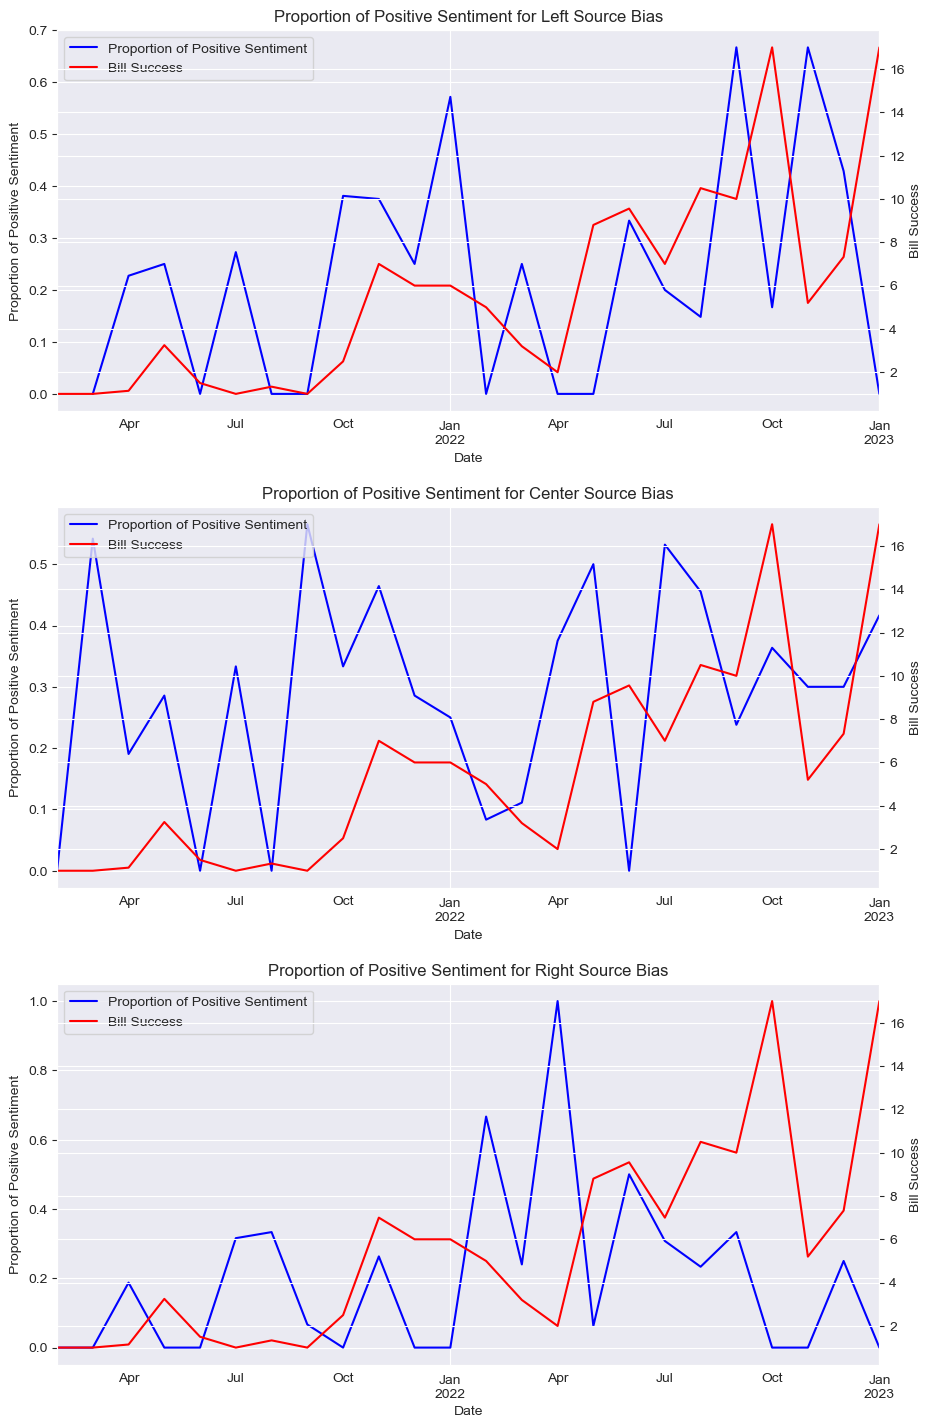
\includegraphics[width=\textwidth]{./figs/fig_10.png}
\begin{pyin}
\## Assume we have the following data available:
# - merged_sentiment_df: DataFrame with 'id', 'sentiment', and 'date' columns
# - bias_df: DataFrame with 'id', 'bias' (or 'bias_label') column
# - bill_data: dictionary with bill information including 'last_action_ordinal' (bill success)

# Extract the relevant information from the bill_data dictionary and convert it to a DataFrame
bill_df = pd.DataFrame(bill_data).T
bill_df['id'] = bill_df['bill_id']  # Create an 'id' column to match with merged_sentiment_df and bias_df

# Merge sentiment_df with bias_df to get bias information
sentiment_bias_df = pd.merge(merged_sentiment_df, bias_df[['id', 'bias']], on='id', how='inner')

# Merge sentiment_bias_df with bill_df to get bill success information
data = pd.merge(sentiment_bias_df, bill_df[['id', 'last_action_ordinal']], on='id', how='inner')

# Rename columns for clarity
data.rename(columns={'bias': 'bias_label', 'last_action_ordinal': 'bill_success'}, inplace=True)

# Print the first few rows of the resulting DataFrame
print(data.head())
\end{pyin}

\begin{pyprint}
Empty DataFrame
Columns: [id, sentiment, bias_label, bias_label, bill_success]
Index: []
\end{pyprint}

\begin{pyin}
import pandas as pd
from sklearn.linear_model import LinearRegression
from sklearn.model_selection import train_test_split
from sklearn.metrics import mean_squared_error
from sklearn.preprocessing import OneHotEncoder

# Assume we have a DataFrame named 'data' containing 'sentiment', 'bias', and 'bill_success' columns
# data = ...

# Convert 'sentiment' and 'bias' columns into one-hot encoded variables
encoder = OneHotEncoder()
sentiment_encoded = encoder.fit_transform(data[['sentiment']]).toarray()
bias_encoded = encoder.fit_transform(data[['bias']]).toarray()

# Combine the one-hot encoded variables into the feature matrix X
X = pd.concat([pd.DataFrame(sentiment_encoded), pd.DataFrame(bias_encoded)], axis=1)

# Define the target variable y (bill_success)
y = data['bill_success']

# Split the data into training and testing sets
X_train, X_test, y_train, y_test = train_test_split(X, y, test_size=0.2, random_state=42)

# Initialize the Linear Regression model
regressor = LinearRegression()

# Train the model on the training data
regressor.fit(X_train, y_train)

# Make predictions on the testing data
y_pred = regressor.predict(X_test)

# Evaluate the model's performance using Mean Squared Error (MSE)
mse = mean_squared_error(y_test, y_pred)
print("Mean Squared Error:", mse)

# You can also evaluate the model's performance using other metrics and interpret the results

\end{pyin}

%%%%%%%%%%%%%%%%%%%%%%%%%%%%%%%%%%%%%%%%%%%%%%%%%%%%%
% ## Intermission
%%%%%%%%%%%%%%%%%%%%%%%%%%%%%%%%%%%%%%%%%%%%%%%%%%%%%

\begin{pyin}
\## load bias data ../data/documents_bias.json
ordinal_bias = ['Left', 'Left-Center', 'Least Biased', 'Right-Center', 'Right']
bias_text = {float(i+1): bias for i, bias in enumerate(ordinal_bias)}
bias_text[None] = None

with open('../data/documents_bias.json') as f:
    bias_data = {doc_id: bias_text[doc['bias_rating']] for doc_id, doc in json.load(f).items()}

# Convert the bias_data dictionary into a DataFrame
bias_df = pd.DataFrame(list(bias_data.items()), columns=['doc_id', 'bias'])
\end{pyin}

\begin{pyin}
\## load sentiment data ../data/all_windows_classified.json
with open('../data/all_windows_classified.json') as f:
    instances = json.load(f)

ordinal_sentiment = ['positive', 'neutral', 'negative']
sentiment_data = {}

for instance_id, instance in instances.items():
    doc_id = instance_id.split('_')[0]
    sentiment = max(instance['sentiment'], key=instance['sentiment'].get)
    sentiment_data[instance_id] = {
        'doc_id': doc_id,
        'sentiment': sentiment
    }

# Convert the sentiment_data dictionary into a DataFrame
sentiment_df = pd.DataFrame(sentiment_data).T.reset_index()
sentiment_df.columns = ['instance_id', 'doc_id', 'sentiment']
\end{pyin}

\begin{pyin}
with open('../data/all_instances_with_bill.json', 'r') as f:
    inst_with_bill = json.load(f)

bill_id_df = pd.DataFrame.from_dict(inst_with_bill, orient='index')
bill_id_df = bill_id_df[['bill_id']]
\end{pyin}

\begin{pyin}
with open('../data/bill_data.json', 'r') as f:
    bill_data = json.load(f)

bill_data_df = pd.DataFrame.from_dict(bill_data, orient='index')
bill_data_df = bill_data_df[['last_action_ordinal', 'last_action_timestamp']]
\end{pyin}

\begin{pyin}
\## Merge the sentiment_df and bias_df DataFrames based on the doc_id column
merged_df = pd.merge(sentiment_df, bias_df, on='doc_id', how='inner')

# Set the 'instance_id' column as the index of the merged_df DataFrame
merged_df.set_index('instance_id', inplace=True)

# merge in bill ids
merged_df = pd.merge(bill_id_df, merged_df, left_index=True, right_on='instance_id')

# merge in bill success
merged_df = pd.merge(bill_data_df, merged_df, left_index=True, right_on='bill_id')

# Rename the 'last_action_ordinal' column to 'bill_success'
merged_df.rename(columns={'last_action_ordinal': 'bill_success'}, inplace=True)
\end{pyin}

\begin{pyin}
merged_df.head()
\end{pyin}

\begin{pyprint}
              bill_success  last_action_timestamp     bill_id      doc_id  \
instance_id                                                                 
5184139624_1            17             1672902000   s4439-117  5184139624   
5137633352_0            17             1672902000   s4439-117  5137633352   
3778807697_0            17             1672902000   s4439-117  3778807697   
3778844056_0            17             1672902000   s4439-117  3778844056   
3290342068_9             6             1672383600  hr2348-117  3290342068   

             sentiment         bias  
instance_id                          
5184139624_1   neutral         None  
5137633352_0   neutral         None  
3778807697_0   neutral  Left-Center  
3778844056_0   neutral         None  
3290342068_9   neutral         None
\end{pyprint}

\begin{pyin}
from pandas.api.types import CategoricalDtype

# Define the ordering of the bias categories
bias_ordering = ['Left', 'Left-Center', 'Least Biased', 'Right-Center', 'Right']
bias_dtype = CategoricalDtype(categories=bias_ordering, ordered=True)

# Convert the 'bias' column to an ordinal categorical variable
merged_df['bias'] = merged_df['bias'].astype(bias_dtype)

# Define the ordering of the bill_success categories (based on your data, modify as needed)
bill_success_ordering = sorted(merged_df['bill_success'].unique())
bill_success_dtype = CategoricalDtype(categories=bill_success_ordering, ordered=True)

# Convert the 'bill_success' column to an ordinal categorical variable
merged_df['bill_success'] = merged_df['bill_success'].astype(bill_success_dtype)

# Convert the 'last_action_timestamp' column to a Pandas date (datetime object)
merged_df['last_action_timestamp'] = pd.to_datetime(merged_df['last_action_timestamp'], unit='s')
\end{pyin}

\begin{pyin}
\## Remove rows with missing values in the 'bias' column
merged_df_clean = merged_df.dropna(subset=['bias'])

# Check the number of remaining rows after removing rows with missing values
print("Number of rows after removing missing values:", merged_df_clean.shape[0])

# Continue with encoding and regression analysis using 'merged_df_clean'
\end{pyin}

\begin{pyprint}
Number of rows after removing missing values: 1723
\end{pyprint}

\begin{pyin}
\## Import the necessary libraries
import statsmodels.api as sm
from sklearn.preprocessing import OneHotEncoder

# Prepare the predictor variables (bias and sentiment as dummy variables)
enc = OneHotEncoder(drop='first', sparse_output=False)  # 'drop' parameter ensures reference category is dropped
X = merged_df_clean[['bias', 'sentiment']]
X_encoded = enc.fit_transform(X)

# Prepare the target variable and encode it as ordinal
# Use 'bill_success' as target variable
y = merged_df_clean['bill_success'].astype(int)

# Create an ordinal logistic regression model
logit_model = sm.MNLogit(y, sm.add_constant(X_encoded))

# Fit the model to the data
result = logit_model.fit()

# Print the summary of the model
print(result.summary())
\end{pyin}

\begin{pyprint}
C:\Users\bessex\AppData\Local\mambaforge\envs\climate-policy\lib\site-packages\sklearn\preprocessing\_encoders.py:868: FutureWarning: `sparse` was renamed to `sparse_output` in version 1.2 and will be removed in 1.4. `sparse_output` is ignored unless you leave `sparse` to its default value.
  warnings.warn(
C:\Users\bessex\AppData\Local\mambaforge\envs\climate-policy\lib\site-packages\statsmodels\discrete\discrete_model.py:2299: RuntimeWarning: overflow encountered in exp
  eXB = np.column_stack((np.ones(len(X)), np.exp(X)))
C:\Users\bessex\AppData\Local\mambaforge\envs\climate-policy\lib\site-packages\statsmodels\discrete\discrete_model.py:2300: RuntimeWarning: invalid value encountered in divide
  return eXB/eXB.sum(1)[:,None]
\end{pyprint}

\begin{pyprint}
Optimization terminated successfully.
         Current function value: nan
         Iterations 4
                          MNLogit Regression Results                          
==============================================================================
Dep. Variable:           bill_success   No. Observations:                 1723
Model:                        MNLogit   Df Residuals:                     1618
Method:                           MLE   Df Model:                           90
Date:                Wed, 12 Apr 2023   Pseudo R-squ.:                     nan
Time:                        14:52:01   Log-Likelihood:                    nan
converged:                       True   LL-Null:                       -2665.3
Covariance Type:            nonrobust   LLR p-value:                       nan
===================================================================================
 bill_success=1       coef    std err          z      P>|z|      [0.025      0.975]
-----------------------------------------------------------------------------------
const                  nan        nan        nan        nan         nan         nan
x1                     nan        nan        nan        nan         nan         nan
x2                     nan        nan        nan        nan         nan         nan
x3                     nan        nan        nan        nan         nan         nan
x4                     nan        nan        nan        nan         nan         nan
x5                     nan        nan        nan        nan         nan         nan
x6                     nan        nan        nan        nan         nan         nan
-----------------------------------------------------------------------------------
bill_success=2       coef    std err          z      P>|z|      [0.025      0.975]
----------------------------------------------------------------------------------
const                 nan        nan        nan        nan         nan         nan
x1                    nan        nan        nan        nan         nan         nan
x2                    nan        nan        nan        nan         nan         nan
x3                    nan        nan        nan        nan         nan         nan
x4                    nan        nan        nan        nan         nan         nan
x5                    nan        nan        nan        nan         nan         nan
x6                    nan        nan        nan        nan         nan         nan
----------------------------------------------------------------------------------
bill_success=3       coef    std err          z      P>|z|      [0.025      0.975]
----------------------------------------------------------------------------------
const                 nan        nan        nan        nan         nan         nan
x1                    nan        nan        nan        nan         nan         nan
x2                    nan        nan        nan        nan         nan         nan
x3                    nan        nan        nan        nan         nan         nan
x4                    nan        nan        nan        nan         nan         nan
x5                    nan        nan        nan        nan         nan         nan
x6                    nan        nan        nan        nan         nan         nan
----------------------------------------------------------------------------------
bill_success=5       coef    std err          z      P>|z|      [0.025      0.975]
----------------------------------------------------------------------------------
const                 nan        nan        nan        nan         nan         nan
x1                    nan        nan        nan        nan         nan         nan
x2                    nan        nan        nan        nan         nan         nan
x3                    nan        nan        nan        nan         nan         nan
x4                    nan        nan        nan        nan         nan         nan
x5                    nan        nan        nan        nan         nan         nan
x6                    nan        nan        nan        nan         nan         nan
----------------------------------------------------------------------------------
bill_success=6       coef    std err          z      P>|z|      [0.025      0.975]
----------------------------------------------------------------------------------
const                 nan        nan        nan        nan         nan         nan
x1                    nan        nan        nan        nan         nan         nan
x2                    nan        nan        nan        nan         nan         nan
x3                    nan        nan        nan        nan         nan         nan
x4                    nan        nan        nan        nan         nan         nan
x5                    nan        nan        nan        nan         nan         nan
x6                    nan        nan        nan        nan         nan         nan
----------------------------------------------------------------------------------
bill_success=7       coef    std err          z      P>|z|      [0.025      0.975]
----------------------------------------------------------------------------------
const                 nan        nan        nan        nan         nan         nan
x1                    nan        nan        nan        nan         nan         nan
x2                    nan        nan        nan        nan         nan         nan
x3                    nan        nan        nan        nan         nan         nan
x4                    nan        nan        nan        nan         nan         nan
x5                    nan        nan        nan        nan         nan         nan
x6                    nan        nan        nan        nan         nan         nan
----------------------------------------------------------------------------------
bill_success=8       coef    std err          z      P>|z|      [0.025      0.975]
----------------------------------------------------------------------------------
const                 nan        nan        nan        nan         nan         nan
x1                    nan        nan        nan        nan         nan         nan
x2                    nan        nan        nan        nan         nan         nan
x3                    nan        nan        nan        nan         nan         nan
x4                    nan        nan        nan        nan         nan         nan
x5                    nan        nan        nan        nan         nan         nan
x6                    nan        nan        nan        nan         nan         nan
----------------------------------------------------------------------------------
bill_success=9       coef    std err          z      P>|z|      [0.025      0.975]
----------------------------------------------------------------------------------
const                 nan        nan        nan        nan         nan         nan
x1                    nan        nan        nan        nan         nan         nan
x2                    nan        nan        nan        nan         nan         nan
x3                    nan        nan        nan        nan         nan         nan
x4                    nan        nan        nan        nan         nan         nan
x5                    nan        nan        nan        nan         nan         nan
x6                    nan        nan        nan        nan         nan         nan
----------------------------------------------------------------------------------
bill_success=10       coef    std err          z      P>|z|      [0.025      0.975]
-----------------------------------------------------------------------------------
const                  nan        nan        nan        nan         nan         nan
x1                     nan        nan        nan        nan         nan         nan
x2                     nan        nan        nan        nan         nan         nan
x3                     nan        nan        nan        nan         nan         nan
x4                     nan        nan        nan        nan         nan         nan
x5                     nan        nan        nan        nan         nan         nan
x6                     nan        nan        nan        nan         nan         nan
-----------------------------------------------------------------------------------
bill_success=11       coef    std err          z      P>|z|      [0.025      0.975]
-----------------------------------------------------------------------------------
const                  nan        nan        nan        nan         nan         nan
x1                     nan        nan        nan        nan         nan         nan
x2                     nan        nan        nan        nan         nan         nan
x3                     nan        nan        nan        nan         nan         nan
x4                     nan        nan        nan        nan         nan         nan
x5                     nan        nan        nan        nan         nan         nan
x6                     nan        nan        nan        nan         nan         nan
-----------------------------------------------------------------------------------
bill_success=12       coef    std err          z      P>|z|      [0.025      0.975]
-----------------------------------------------------------------------------------
const                  nan        nan        nan        nan         nan         nan
x1                     nan        nan        nan        nan         nan         nan
x2                     nan        nan        nan        nan         nan         nan
x3                     nan        nan        nan        nan         nan         nan
x4                     nan        nan        nan        nan         nan         nan
x5                     nan        nan        nan        nan         nan         nan
x6                     nan        nan        nan        nan         nan         nan
-----------------------------------------------------------------------------------
bill_success=14       coef    std err          z      P>|z|      [0.025      0.975]
-----------------------------------------------------------------------------------
const                  nan        nan        nan        nan         nan         nan
x1                     nan        nan        nan        nan         nan         nan
x2                     nan        nan        nan        nan         nan         nan
x3                     nan        nan        nan        nan         nan         nan
x4                     nan        nan        nan        nan         nan         nan
x5                     nan        nan        nan        nan         nan         nan
x6                     nan        nan        nan        nan         nan         nan
-----------------------------------------------------------------------------------
bill_success=15       coef    std err          z      P>|z|      [0.025      0.975]
-----------------------------------------------------------------------------------
const                  nan        nan        nan        nan         nan         nan
x1                     nan        nan        nan        nan         nan         nan
x2                     nan        nan        nan        nan         nan         nan
x3                     nan        nan        nan        nan         nan         nan
x4                     nan        nan        nan        nan         nan         nan
x5                     nan        nan        nan        nan         nan         nan
x6                     nan        nan        nan        nan         nan         nan
-----------------------------------------------------------------------------------
bill_success=16       coef    std err          z      P>|z|      [0.025      0.975]
-----------------------------------------------------------------------------------
const                  nan        nan        nan        nan         nan         nan
x1                     nan        nan        nan        nan         nan         nan
x2                     nan        nan        nan        nan         nan         nan
x3                     nan        nan        nan        nan         nan         nan
x4                     nan        nan        nan        nan         nan         nan
x5                     nan        nan        nan        nan         nan         nan
x6                     nan        nan        nan        nan         nan         nan
-----------------------------------------------------------------------------------
bill_success=17       coef    std err          z      P>|z|      [0.025      0.975]
-----------------------------------------------------------------------------------
const                  nan        nan        nan        nan         nan         nan
x1                     nan        nan        nan        nan         nan         nan
x2                     nan        nan        nan        nan         nan         nan
x3                     nan        nan        nan        nan         nan         nan
x4                     nan        nan        nan        nan         nan         nan
x5                     nan        nan        nan        nan         nan         nan
x6                     nan        nan        nan        nan         nan         nan
===================================================================================
\end{pyprint}

%%%%%%%%%%%%%%%%%%%%%%%%%%%%%%%%%%%%%%%%%%%%%%%%%%%%%
%%%%%%%%%%%%%%%%%%%%%%%%%%%%%%%%%%%%%%%%%%%%%%%%%%%%%
